\documentclass[11pt]{article}
\def\nterm {Autumn}
\def\nyear {2022}
\def\nlecturer {D. Papageorgiou, V. Shahrezaei}
\def\ncourse {Calculus and Application}
\def\nshort {Calculus and Application}
\usepackage{amsmath, amsthm, amssymb, amsfonts}
\usepackage{fancyhdr}
\usepackage{xparse, xpatch}
\usepackage[svgnames]{xcolor}
\usepackage[shortlabels]{enumitem}
\usepackage[thinc,text]{esdiff}
\usepackage[bottom]{footmisc}
\usepackage[most]{tcolorbox}
\usepackage{physics}
\usepackage{tikz}
\usepackage{pgfplots}
\usepackage{graphicx, tabularx, caption}
\usepackage{csquotes}
\usepackage[a4paper, left=1.2in, right=1.2in, bottom=1in]{geometry}
\usepackage[hidelinks]{hyperref}
\hypersetup{
    colorlinks,
    allcolors=black
}
\pgfplotsset{compat=1.18}
\graphicspath{{./images/}}

% meta
\setlength{\headheight}{13.6pt}
\renewcommand*\contentsname{Outline}
\pagestyle{fancy}
\lhead{\nouppercase{\leftmark{}}}
\rhead{\nshort}
\title{\textbf{\ncourse}}
\author{Lectured by \nlecturer \\\small Notes taken by Dongshen Wu\footnote{These notes are usually modified significantly after lectures, and are not endorsed by the lecturers at Imperial College, London. They are by no means an accurate representations of what was actually lectured. In particular, all errors are almost surely mine.}}
\date{\nterm \nyear}

% centre tikz pictures
\makeatletter
\g@addto@macro\@floatboxreset\centering
\makeatother

% environment
\tcbset{
  defstyle/.style={
    enhanced, sharp corners,
    attach boxed title to top left={yshift=-2.75mm, 
      xshift=5mm, yshifttext=-2.2mm},
    colback=white, colframe=PeachPuff,
    coltitle=black, fonttitle=\bfseries,
    before skip=7pt,
    boxed title style={sharp corners, size=small,
      colback=PeachPuff,colframe=PeachPuff,}},
  thmstyle/.style={
    enhanced, sharp corners,
    attach boxed title to top left={yshift=-2.75mm, 
      xshift=5mm, yshifttext=-2.2mm},
    colback=AliceBlue, colframe=LightBlue,
    coltitle=black, fonttitle=\bfseries,
    before skip=7pt,
    boxed title style={sharp corners, size=small,
      colback=LightBlue,colframe=LightBlue,}},
  propstyle/.style={
    enhanced, sharp corners,
    attach boxed title to top left={yshift=-2.75mm, 
      xshift=5mm, yshifttext=-2.2mm},
    colback=white, colframe=PowderBlue,
    coltitle=black, fonttitle=\bfseries,
    before skip=7pt,
    boxed title style={sharp corners, size=small,
      colback=PowderBlue,colframe=PowderBlue,}},
}

\newtcbtheorem[number within=section]{TcbThm}{Theorem}{
  thmstyle}{thm}
\NewDocumentEnvironment{theorem}{ O{} O{} }
  {\TcbThm{#1}{#2}}{\endTcbThm}

\newtcbtheorem[number within=section, use counter from=TcbThm]{TcbProp}{Proposition}{
  propstyle}{prop}
\NewDocumentEnvironment{proposition}{ O{} O{} }
  {\TcbProp{#1}{#2}}{\endTcbProp}

\newtcbtheorem[number within=section,use counter from=TcbThm]{TcbDef}{Definition}{
  defstyle}{def}
\NewDocumentEnvironment{definition}{ O{} O{} }
  {\TcbDef{#1}{#2}}{\endTcbDef}

\newtcbtheorem[number within=section,use counter from=TcbThm]{TcbAxi}{Axiom}{
  defstyle}{axi}
\NewDocumentEnvironment{axiom}{ O{} O{} }
  {\TcbAxi{#1}{#2}}{\endTcbAxi}

\newtheorem{corollary}[\tcbcounter]{Corollary}
\tcolorboxenvironment{corollary}{propstyle}
\newtheorem{lemma}[\tcbcounter]{Lemma}
\tcolorboxenvironment{lemma}{propstyle}

\theoremstyle{definition}
\newtheorem*{example}{Example}
\newtheorem*{exercise}{Exercise}
\newtheorem{problem}{Problem}
\newtheorem*{algorithm}{Algorithm}
\newtheorem*{procedure}{Procedure}
\newtheorem*{remark}{Remark}
\tcolorboxenvironment{algorithm}{propstyle}

\theoremstyle{remark}
\newtheorem*{notation}{Notation}
\newtheorem*{solution}{Solution}
\tcolorboxenvironment{solution}{
  blanker,breakable,left=5mm,
  before skip=10pt,after skip=10pt,
  parbox = false,
  borderline west={0.5mm}{0pt}{SlateGray}}
\tcolorboxenvironment{proof}{
  blanker,breakable,left=5mm,
  before skip=10pt,after skip=10pt,
  parbox = false,
  borderline west={0.5mm}{0pt}{SlateGray}}

\newtcolorbox{extension}[1]{
  colback=WhiteSmoke,colframe=Gainsboro, enhanced, before skip=10pt, after skip=10pt, fonttitle=\bfseries,coltitle=black, sharp corners, title={\:\,Extension:\:#1}, before upper app={\setlength{\parindent}{17pt}}
}

% subproof
\makeatletter
\newcounter{subproof}
\xpretocmd{\proof}{\setcounter{subproof}{0}}{}{}
\xpretocmd{\solution}{\setcounter{subproof}{0}}{}{}
\newcommand{\subproof}[1]{%
  \par
  \addvspace{\medskipamount}%
  \stepcounter{subproof}%
  \noindent\emph{Part \thesubproof: #1}\par\nobreak
  \@afterheading
}
\makeatother

% command
\newcommand{\C}{\mathbb{C}}
\newcommand{\N}{\mathbb{N}}
\newcommand{\Q}{\mathbb{Q}}
\newcommand{\R}{\mathbb{R}}
\newcommand{\Z}{\mathbb{Z}}
\renewcommand{\bf}[1]{\mathbf{#1}}
\renewcommand{\cal}[1]{\mathcal{#1}}
\renewcommand{\rm}[1]{\mathrm{#1}}
\newcommand{\floor}[1]{\left \lfloor #1 \right \rfloor}
\newcommand{\ceil}[1]{\left \lceil #1 \right \rceil}
\newcommand{\lointerval}[1]{\ensuremath{\left(#1\right]}}
\newcommand{\rointerval}[1]{\ensuremath{\left[#1\right)}}
% Augmented Matrix
\newenvironment{amatrix}[1]{%
  \left(\begin{array}{@{}*{#1}{c}|c@{}}
}{%
  \end{array}\right)
}

\begin{document}
\maketitle{}
\tableofcontents{}
\pagebreak

%=========================================================
\section{Limits and Continuity}
\subsection{Formal definition of limits}
For this session we shall consider numbers in the reals. We are concerned about the behaviour of function \(f(x)\) near a point \(x_0\). Suppose that this function is well-defined at all points near \(x_0\), except possibly at \(x_0\), then
\begin{definition}[Epsilon-Delta]
  We say that \(l\) is the limit of \(f(x)\) as \(x\) approaches \(x_0\) if: for all \(\epsilon >0\), there exists \(\delta > 0\), such that \(|f(x)-l|<\epsilon\) for all \(|x-x_0|<\delta\) and \(x \neq x_0\). 
  
  We denote this as \(\lim_{x\to x_0}f(x)=l\).
\end{definition}

\begin{example}
  Show that \(\lim_{x\to2}\sqrt{x} = \sqrt{2}\) using \(\epsilon-\delta\) definition of limit.
\end{example}
\begin{solution}
  Given \(\epsilon > 0\), we need to find \(\delta>0\) such that \(|\sqrt{x}-\sqrt{2}|<\epsilon\) whenever \(|x-2|<\delta\). Note that for all \(x>0\) we have,
  \[|\sqrt{x}-\sqrt{2}|=\frac{|x-2|}{\sqrt{x}+\sqrt{2}}|\leq \frac{|x-2|}{\sqrt{2}}\]
  so pick \(\delta = \sqrt{2}\epsilon\) will do.
\end{solution}

\begin{proposition}[Properties of limits]
  If both \(\lim_{x\to x_0}f(x)\) and \(\lim_{x\to x_0}g(x)\) exists, and \(h(x)\) continuous at limit, then
  \begin{itemize}
    \item \(\lim_{x\to x_0}[f(x)+g(x)] = \lim_{x\to x_0}f(x) + \lim_{x\to x_0}g(x)\)
    \item \(\lim_{x\to x_0}[f(x) \cdot g(x)] = \lim_{x\to x_0}f(x) \cdot \lim_{x\to x_0}g(x)\)
    \item \(\lim_{x\to x_0}[f(x)/g(x)] = \lim_{x\to x_0}f(x) / \lim_{x\to x_0}g(x)\)
    \item \(\lim_{x\to x_0}h(f(x)) = h(\lim_{x\to x_0}f(x))\)
  \end{itemize}
\end{proposition}

The properties above in fact holds when either \(x_0\) or \(l\) approaches infinity.
\begin{definition}[Epsilon-A]
  Let \(f(x)\) be well defined on \(a,\infty\) and \(l\) a real number. Then \(\lim_{x\to\infty}f(x)=l\) if: for all \(\epsilon>0\), there exists a \(A>a\), such that \(|f(x)-l|<\epsilon\) for all \(x>A\). Analogus for negative.
\end{definition}

\begin{definition}[B-Epsilon]
  We say \(\lim_{x\to x_0}f(x)=\infty\) if: for all \(B>0\), there exists \(\epsilon>0\), such that \(f(x)>B\) for all \(|x-x_0|<\epsilon\) and \(x\neq x_0\). This is in some sense the `reverse' of the previous statement.
\end{definition}

Sometimes the limit at \(x_0\) could be different depending on which side you approach it from, e.g. \(f(x)=1/x\) and \(x_0=0\), so let's define one-sided limits. It is very similar to the normal definition, except \(\delta\) only restricts from one side.

\begin{definition}[One-sided limit]
  We say that \(\lim_{x\to x_0 +}f(x)=l\) (from the right) if: for all \(\epsilon >0\), there exists \(\delta > 0\), such that \(|f(x)-l|<\epsilon\) for all \(x_0<x<x_0+\delta\). Analogus for left.
\end{definition}

\begin{proposition}[Comparison test for limits]
  If \(\lim_{x\to x_0}f(x)=0\) and \(|g(x)|\leq|f(x)|\) for all \(x\) near \(x_0\) but not equal to \(x_0\) (large enough \(x\) for \(x_0 \to \infty\)), then \(lim_{x\to x_0}g(x)=0\).
\end{proposition}

%----------------------------------------------------
\subsection{Continuity}

\begin{definition}[Continuity]
  We say that \(f\) is continuous at \(x_0\) if \(\lim_{h\to 0}f(x_0+h)=f(x_0)\) or equivalently \(\lim_{x\to x_0}f(x)=f(x_0)\).
\end{definition}
Note that the first version look very much like the definition of derivative.  

Sometimes functions may be very nice everywhere except from a few points, such as:
\[f(x)=\sin \left(\frac{1}{x} \right)\]
\[f(x)=x\sin \left(\frac{1}{x} \right)\]

The question is: can we define \(f(0)\) so that the function is continuous.

We can easily see from a graph that the first is not possible as it oscillates infinitely and takes all values from \(-1\) to \(1\). The \(\epsilon - \delta\) definition would never be satisfied.

However, we may define \(f(0)=0\) for the second one. Then, continuity is guaranteed:
\[|x\sin \left(\frac{1}{x}\right)-0| \leq |x| < \epsilon, \forall |x|\leq \epsilon\]

%----------------------------------------------------
\subsection{Indeterminate form}
Limits involving an algebraic combination of functions in an independent variable may often be evaluated by replacing these functions by their limits; if the expression obtained after this substitution does not provide sufficient information to determine the original limit, then the expression is called an indeterminate form. The most common ones are
\[\frac{0}{0}, \frac{\infty}{\infty}, 0\cdot\infty, \infty-\infty, 0^0, 1^\infty, \infty^0\]

A really useful tool for evaluating them is the L'Hopital Rule.

\begin{theorem}[L'Hopital's Rule (Special)]
  Consider \(f,g\) continuously differentiable on an open interval containgin \(c\), and \(g'(x)\neq 0\).
  If \(\lim_{x\to c}f(x) = \lim_{x\to c}f(x) = 0 \text{ or } \pm\infty\), then
  \begin{equation*}
    \lim_{x\to c}\frac{f(x)}{g(x)} = \lim_{x\to c}\frac{f'(x)}{g'(x)} 
  \end{equation*}
  Note that \(c\) can be \(\pm\infty\) too.
\end{theorem}
\begin{proof}
  We have \(f(c)=g(c)=0\) and \(g'(c)\neq 0\). Then
  \begin{equation*}
    \lim_{x\to c}\frac{f(x)}{g(x)} = \lim_{x\to c}\frac{f(x)-f(c)}{g(x)-g(c)} = \frac{\lim_{x\to c}\frac{f(x)-f(c)}{x-c}}{\lim_{x\to c}\frac{g(x)-g(c)}{x-c}} = \frac{f'(c)}{g'(c)} = \lim_{x\to c}\frac{f'(x)}{g'(x)}
  \end{equation*}
\end{proof}
For functions not of the form required, we can often transform them using reciprocal, exponentiation, and logarithm.

We also introduce the idea of equivalent infinitesimal.
\begin{definition}[Equivalent Infinitesimal]
  When two variables \(x,y\) converge to \(0\) at the same limit point and \(\lim\frac{y}{x}=1\), they are called equivalent infinitesimal, denoted as \(x \sim y\).
\end{definition}
\begin{proposition}[Common equivalent infinitesimal]
  \(x \sim \sin(x) \sim \arcsin(x) \sim \sinh(x) \sim \tan(x) \sim \arctan(x) \sim \ln(1+x), 1-\cos(x) \sim \frac{x^2}{2}\)
\end{proposition}

%=========================================================
\section{Diffrentiation}
\subsection{Derivative}
\begin{definition}[Differentiability]
  A function \(f\) is differentiable at \(x_0\) if the `Newton quotient'
  \begin{equation*}
    \lim_{h\to 0}\frac{f(x_0+h)-f(x_0)}{h} = \lim_{h\to 0}\frac{f(x_0+h)-f(x_0-h)}{2h}
  \end{equation*}
  exists. We call this \(f'(x_0)\), the derivative of \(f\) at a point \(x_0\).
  
  If we replace \(h=x-x_0\), we get the equivalent definition of 
  \[f'(x_0)=\lim_{x\to x_0}\frac{f(x)-f(x_0)}{x-x_0}\]
\end{definition}

The latter is in fact more computationally efficient than the former (complexity of \(O(h^2)\) as oppose to \(O(h)\)).

\begin{proposition}[Properties of derivative]
  \begin{enumerate}
    \item \((cf)'(x)=cf'(x)\)
    \item \((f+g)'(x)=f'(x)+g'(x)\)
  \end{enumerate}
\end{proposition}

\begin{proposition}[Product rule]
  For \(f,g\) differentiable, \(\diff{}{x}f(x)g(x)=f'(x)g(x)+g'(x)f(x)\).
\end{proposition}
\begin{proof}
  \begin{align*}
    (f(x)g(x))' &= \lim_{h\to 0}\frac{f(x+h)g(x+h)-f(x)g(x)}{h} \\
    &= \lim_{h\to 0}\frac{f(x+h)g(x+h)-f(x+h)g(x)+f(x+h)g(x)-f(x)g(x)}{h} \\
    &= \lim_{h\to 0}f(x+h)\frac{g(x+h)-g(x)}{h} + \lim_{h\to 0}g(x)\frac{f(x+h)-f(x)}{h} \\
    &=f(x)g'(x)+g(x)f'(x)
  \end{align*}
\end{proof}

\begin{proposition}[Chain rule]
  For \(f,g\) differentiable, \(\diff{}{x}f(g(x))=f'(g(x))g'(x)\)
\end{proposition}
\begin{proof}
  Using the definition, we have
  \begin{align*}
    (f\circ g)'(x) &= \lim_{h\to 0}\frac{fg(x+h)- fg(x)}{h} \\
    &= \lim_{h\to 0}\frac{fg(x+h)-fg(x)}{g(x+h)-g(x)}\cdot \frac{g(x+h)-g(x)}{h}
  \end{align*}
  Let \(k=g(x+h)-g(x)\) and \(u=g(x)\), so \(k \to 0\) when \(h \to 0\), then
  \begin{align*}
    (f\circ g)'(x) &= \lim_{h\to 0}\frac{f(u+k)-f(u)}{k}\cdot \frac{g(x+h)-g(x)}{h}\\
    &= \lim_{k\to 0}\frac{f(u+k)-f(u)}{k}\cdot \lim_{h\to 0}\frac{g(x+h)-g(x)}{h} \\
    &= f'(u)g'(x) = f'(g(x))g'(x)
  \end{align*}
\end{proof}
The quotient rule can be derived using chain rule and product rule.

Implicit differentiation simply refers to the fact that we treat \(y(x)\) and its derivative as a function that we do not know explicitly.

Here is an example of related rate of change using implicit differentiation.
\begin{example}
  The surface area of a cube is growing at a constant rate of \(4cm^2/s\). How fast is the
  length of a side growing when the cube sides are \(2cm\) long? Find the side length when
  the rate of change of the volume exceeds that of the area.\(\dv[n]{f}{x}\)
\end{example}
\begin{solution}
  Note \(A=6x^2\), so \(\diff{A}{t}=12x\diff{x}{t}=4\), i.e. \(\diff{x}{t}=\frac{1}{3x}\). Hence \(\left.\diff{x}{t}\right\rvert_{x=2}=\frac{1}{6}\).

  Similarly, \(V=x^3\) so \(\diff{V}{t}=3x^2\diff{x}{t}=\frac{x}{4}\diff{A}{t}\). Hence \(\diff{V}{t}>\diff{A}{t}\) numerically when \(x>4\).
\end{solution}

\begin{proposition}
  If \(f(x)\) is differentiable at \(x_0\), then it is also continuous here.
\end{proposition}
\begin{proof}
  \begin{equation*}
    \lim_{x\to x_0}(f(x)-f(x_0)) = \lim_{x\to x_0}\frac{f(x)-f(x_0)}{x-x_0}\cdot (x-x_0) = f'(x_0)\cdot 0 = 0
  \end{equation*}
\end{proof}
It follows (by contrapositive) that \(f\) is not differentiable it it is not continuous at \(x_0\).

\begin{exercise}
  Suppose \(f\) is continuous at \(x_0\) and is differentiable at an interval close to \(x_0\) (except possibly at \(x_0\)). Suppose also that \(\lim_{x\to x_0}f'(x)=m\). Show that \(f'(X)\) exists and equals to \(m\).
\end{exercise}
\begin{proof}
  Due to continuity, we have \(\lim_{x\to x_0}f(x)=f(x_0)\). Then we have \[\lim_{x\to x_o}f'(x)-f'(x_0)=\lim\left(\frac{f(x)-f(x_0)}{x-x_0}-m\right)=0\]
  Since \(f\) is differentiable near \(x_0\), by MVT, thre exists \(c\) between \(x,x_0\) such that \[\lim_{x\to x_0}(f'(c)-m)=0\]
  Taking the limits then squeezes \(c\) and gives the result.
\end{proof}

\subsection{Fundamental theorems}
For the proof of these theorems, refer to Analysis notes.

\begin{theorem}[Boundedness Theorem]
  If \(f(x)\) is continuous on \([a,b]\) then it is bounded on \([a,b]\).
\end{theorem}

\begin{theorem}[Extreme Value Theorem]
  If a real-valued function \(f\) is continuous on \([a,b]\), then \(f\) must attain at least one maximum and one minimum. That is, there exist numbers \(c\) and \(d\) in \([a,b]\) such that:
  \[f(c)\geq f(x) \geq f(d), \forall x\in[a,b]\]
\end{theorem}

\begin{theorem}[Rolle's Theorem]
  Let \(f(x)\) be continuous over \([a,b]\) and differentiable over \((a,b)\). If \(f(a)=f(b)\), then there exists a point \(c, a<c<b\) such that \(f'(c)=0\).
\end{theorem}

\begin{theorem}[Mean Value Theorem]
  Suppose \(f(x)\) is continuous on \([a,b]\) and differentiable on \((a,b)\). Then there exists \(a < c < b\) such that 
  \begin{equation*}
    f'(c)=\frac{f(b)-f(a)}{b-a}
  \end{equation*}
\end{theorem}
\begin{proof}
  The straight line joining \((a,f(a))\) and \((b,f(b))\) has equation
  \begin{equation*}
    y(x)=\frac{f(b)-f(a)}{b-a} (x-a)+f(a)
  \end{equation*}
  Consider \(g = f(x) - y(x)\). Then \(g(a)=g(b)=0\), so by Rolle's theorem, there exists \(a<c<b\) such that \(g'(c)=0\).
  But \(g'(x)=f'(x)-\frac{f(b)-f(a)}{b-a}\).
\end{proof}

\begin{theorem}[Intermediate Value Theorem]
  Let \(f\) be continuous on \([a,b]\). Given any number \(y\) between \(f(a)\) and \(f(b)\), there exists a point \(x\) between \(a\) and \(b\) such that \(f(x)=y\).
\end{theorem}

\begin{corollary}[Bolzano's theorem]
  If a continuous function has values of opposite sign inside an interval, then it has a root in that interval.
\end{corollary}

\subsection{Inverse function}
\begin{definition}[Inverse function]
  Let \(y=f(x)\) be defined on some interval. Given any \(y\) in the range of \(f\), if we can find a unique value of \(x\) in its domain such that \(f(x)=y\), then we can define the inverse function as \(x=f^{-1}(y)\).
\end{definition}

\begin{proposition}
  If \(f(x)\) is continuous on \([a,b]\) and is strictly increasing (or decreasing), and \(f(a)=c\) and \(f(b)=d\), then \(x=f^{-1}(y)\) is defined on \([c,d]\).
\end{proposition}

\begin{proposition}
  If \(f\) is differentiable and strictly increasing/decreasing on \((a,b)\), then inverse \(g\) exists and has derivative:
  \begin{equation*}
    g'(y)=\diff{}{y}f^{-1}(y)=\frac{1}{f'(x)}
  \end{equation*}
\end{proposition}
\begin{proof}
  By intermediate value theorem and the fact that it is monotonic, \(g(y)\) well defined for all \(y\in [f(a),f(b)]\), in particular, \(f(x+h)=y+k, g(y+k)=x+h\). Also recall \(f(x)=y, g(y)=x\). Hence we have 
  \[\lim_{k\to 0}\frac{g(y+k)-g(y)}{k} = \lim_{h\to 0}\frac{h}{f(x+h)-f(x)}=\frac{1}{f'(x)}\]
\end{proof}

\subsection{Exponentiation and logarithmic}
\begin{definition}[Exponential function]
  There are few equivalent ways to define the exponential function:
\begin{enumerate}
  \item As a limit \[e^x=\lim_{n\to\infty}\left(1+\frac{x}{n}\right)^n\]
  \item As a power series \[e^x=\sum_{n=0}^\infty\frac{x^n}{n!}\]
  \item As the unique solution to the initial value problem \[y'=y,y(0)=1\]
  \item As the inverse of natural logarithm, i.e. the unique number \(y>0\) such that \[\int_1^y \frac{dt}{t} =x\]
  \item As the unique function satisfying \[f'(0)=1 \text{ and } f(x+y)=f(x)f(y)\]
  \item As the exponential function with the unique base satisfying \[\lim_{h\to 0}\frac{e^h-1}{h}=1 (=ln(e))\]
\end{enumerate}
\end{definition}
See wikipedia for proof of why the characterisations are equivalent.

\begin{definition}[Natural logarithm]
  The natural logarithm \(\ln(x)\) is the inverse function of exponential.
\end{definition}
Of course, we can characterise natural logarithm first in the numerous equivalent ways, such as \(\ln(t)=\int_1^t\frac{dx}{x}\) or the unique increasing function satisfying \(f(xy)=f(x)+f(y)\) and \(f(1)=0\), then define the exponential as its inverse.

\vspace{5pt}We can now make sense of exponential of any base by defining \(b^x=e^{x\ln(b)}\) and similarly, \(\log_b(x)\) can be defined as the number \(y\) such that \(b^y=x\).

\begin{proposition}[Common properties of log]
  \begin{itemize}
    \item \(\log(xy)=\log(x)+\log(y)\)
    \item \(\log(x^y)=y\log(x)\)
    \item \(\log_ba=\frac{\log_ca}{\log_cb}\)
  \end{itemize}
\end{proposition}

\begin{example}[Logarithmic differentiation]
  We may differentiate function of the form \(y=f(x)^{g(x)}\) using logarithmic differentiation. Take the natural logarithm of both sides gives:
  \begin{align*}
    \ln(y) &= g(x)\ln(f(x)) \\
    \frac{y'}{y} &= g'(x)\ln(f(x))+g(x)(\ln(f(x)))' \\
    y' &= f(x)^{g(x)}g'(x)\ln(f(x))+g(x)\frac{f'(x)}{f(x)}
  \end{align*}
\end{example}

\begin{theorem}[Cauchy Mean Value Theorem]
  Let \(f,g\) be continuous on \([a,b]\) and differentiable on \((a,b)\) with \(g(a)\neq g(b)\). Then there exists \(c\) in \((a,b)\) such that
  \[g'(c)\frac{f(b)-f(a)}{g(b)-g(a)}=f'(c)\]
\end{theorem}
\begin{proof}
  Let \[h(x)=f(a)+(g(x)-g(a))\frac{f(b)-f(a)}{g(b)-g(a)}\]
  Then, \(h(a)=f(a), h(b)=f(b)\). For the function \(\phi(x)=h(x)-f(x)\) we have \(\phi(a)=\phi(b)=0\) and \(\phi\) is differentiable on \((a,b)\). By mean value theorem, there exists \(c\in (a,b)\) such that \(\phi '(c) =0\) i.e. \(f'(c)=h'(c)\) as required.
\end{proof}

\begin{theorem}[L'Hopital Rule (General)]
  Let \(\mathcal{I}\) be an open interval contains \(c\). Assume that \(f,g\) are differentiable and \(g'(x)\neq 0\) on the interval \(\mathcal{I}\) except possibly at \(c\). If \(\lim_{x\to c}\frac{f'(x)}{g'(x)}=l\), and \(\lim_{x\to c}f(x) = \lim_{x\to c}f(x) = 0 \text{ or } \pm\infty\), then
  \[\lim_{x\to c}\frac{f(x)}{g(x)} = l\]
\end{theorem}
Note that this is more general than the one previously introduced as it does not require \(f,g\) to be differentiate at \(c\). Also note that \(c,l\) can be taken from the \emph{extended real number line}, \(\R\cup\{\infty,-\infty\}\), which we shall introduce later.
\begin{proof}
  See wikipedia.
\end{proof}

\begin{problem}[Dog chasing rabbit]
  A rabbit moves along the positive \(x\)−axis with constant speed \(\alpha\), and a dog chases the rabbit with constant speed \(\beta\). The rabbit starts at time \(t=0\) at the origin (0, 0) and the dog at \((0,h)\). Find the trajectory described by the dog in its pursuit of the rabbit. The dog always instantaneously aligns its direction of travel along the line joining her position
with the rabbit’s.
\end{problem}
\begin{solution}
  %EXT challenge 1
\end{solution}

\section{Integration}
\subsection{Riemann Integral}
\begin{definition}[Antiderivative]
  Antiderivative of \(f(x)\) is the differentiable function \(F(x)\) such that \[F'(x)=f(x)\]
  We denote \(F(x)=\int f(x) \,dx\) the indefinite integral of \(f\).
\end{definition}
The antiderivative is the opposite of derivative (as suggested by the name), and it is not unique as \(F(x)+c\) is also an antiderivative of \(f(x)\) for arbitrary \(c\in\R\).

\vspace{5pt}Geometrically, the integral of \(f(x)\) with respect to \(x\) represents the \emph{signed area} between the curve and the \(x-axis\), where the area is negative below the axis.

\begin{definition}[Riemann sum]
  Given \(f(x), x\in [a,b]\), partition it into equal sub-intervals:
  \[x_i=a+ih, \:\:\:\:\: i=0,1,...,n, \:\:\:\:\: h=\frac{b-a}{n}\]
  Let \(x_i^* \in [x_{i-1},x_i]\). The Riemann sum is 
  \[\sum_{i=1}^n f(x_i^*)h\]
  Normally we pick \(x_i^*\) as one of the following: \(x_i\) (upper RS); \(x_{i-1}\) (lower RS); or \(\frac{1}{2}(x_{i-1}+x_i)\) (midpoint RS).
\end{definition}
There are more technicality in the formal definition (we don't have to restrict to equal length intervals), but for our purpose this is good enough. 
\begin{definition}[Riemann integral]
  A function \(f\) is said to be \emph{Riemann-integrable} if the limit of the Riemann sum exists as \(n\to\infty\). This limit is the definite Riemann integral.
  \[\lim_{n\to\infty}\sum_{i=1}^n f(x_i^*)h=\int_a^b f(x)\,dx\]
\end{definition}
There is also a more general form of integration called Lebesgue integral, which would be discussed in more details in the measure theory course.

\begin{theorem}[Fundamental Theorem of Calculus (1st part)]
  Let \(f\) be continuous real-valued function defined on \([a,b]\) and \(F\) be defined on the same interval by
  \[F(x)=\int_a^xf(t)\,dt\]
  Then \(F\) is an antiderivative of \(f\).
\end{theorem}
%TODO proof of FTC
\begin{theorem}[Fundamental Theorem of Calculus (2nd part)]
  Let \(f\) be real-valued function defined on \([a,b]\) and \(F\) be its antiderivative. If \(f\) is Riemann-integrable on \([a,b]\), then
  \[\int_a^bf(x)\,dx=F(b)-F(a)\]
\end{theorem}
This is sometimes known as the Newton-Leibniz axiom, and it ``defines'' the definite integral.

\begin{corollary}
  \[\diff{}{x}\int_a^g(x)f(t)\,dt=f(g(x))\cdot g'(x)\]
\end{corollary}

\begin{proposition}[Properties of definite integral]
  \begin{enumerate}
    \item \(\int_a^b cf(x)\,dx=c\int_a^b f(x)\,dx\)
    \item \(\int_a^b (f(x)+g(x))\,dx=\int_a^b f(x)\,dx + \int_a^b g(x)\,dx\)
    \item If \(c\in (a,b)\) then \(\int_a^b f(x)\,dx=\int_a^c f(x)\,dx + \int_c^b f(x)\,dx\)
    \item If \(f(x)\leq g(x)\) for \(x\in [a,b]\), then \(\int_a^b f(x)\,dx \leq \int_a^b g(x)\,dx\)
    \item \(\int_a^b f(x)\,dx=-\int_b^a f(x)\,dx\)
  \end{enumerate}
\end{proposition}

\begin{definition}[Improper integral]
  An integral \(\int_a^bf(x\,dx)\) is improper if
  \begin{enumerate}
    \item \(a=-\infty\) or \(b=\infty\)
    \item \(f(x_0)\to \pm\infty\) for some \(x\in(a,b)\)
  \end{enumerate} 
\end{definition}

We need to consider the limit in these case, e.g. for \(f(x)=\frac{e^{-x}}{\sqrt{x}}\)
\begin{equation}
  \label{eq:1}
  \int_0^\infty f(x)=\lim_{\epsilon\to 0^+}\int_\epsilon^a f(x)\,dx+\lim_{M\to\infty}\int_a^M f(x)\,dx=\lim_{M\to\infty}F(M)-\lim_{\epsilon\to 0^+}F(\epsilon)
\end{equation} 
where \(a\in (0,\infty)\) is arbitrary and \(F(x)\) is the antiderivative.

In the case where integral is inpractical to find, we can use a comparison test to decide whether the integral diverge or converge.
\begin{proposition}[Comparison test]
  Suppose \(f,g\) satisfy \(|f(x)|\leq g(x)\) for all \(x\geq a\) and \(\int_a^b f(x)\,dx, \int_a^b g(x)\,dx \) exists, then
\end{proposition}

\begin{example}
  Here are some example of comparison tests:
  \begin{itemize}
    \item \(\int_0^\infty \frac{\sin(x)}{(1+x)^2}\,dx \leq \int_0^\infty \frac{1}{(1+x^2)}\,dx \leq \int_0^\infty \frac{1}{x^2}\,dx\) which is convergent.
    \item \(\int_1^\infty\frac{dx}{\sqrt{1+x^2}}\geq \int_1^\infty\frac{dx}{\sqrt{x^2+x^2}}=\int_1^\infty \frac{dx}{\sqrt{2}x}\) which is divergent.
  \end{itemize}
\end{example}
\begin{exercise}
  Show the integral in equation \ref{eq:1} is convergent using comparison test.
\end{exercise}

\begin{definition}[Mean values]
  The mean value of \(f(x)\) over \([a,b]\) is defined by
  \[\frac{1}{b-a}\int_a^bf(x)\,dx\]
\end{definition}

\begin{theorem}
  If \(f\) is continuous over \((a,b)\), then there exists \(x_0\in (a,b)\) such that \(f(x_0)\) is equal to the mean value of \(f\).
\end{theorem}
\begin{proof}
  Consider \(F(x)\) the antiderivative of \(f\), which is continuous over \((a,b)\) given \(f\) is. Then by MVT, we have
  \[F'(x_0)=\frac{F(b)-F(a)}{b-a}\]
  which by FTC is 
  \(f(x_0)=\frac{\int_a^bf(t)\,dt-\int_a^af(t)\,dt}{b-a}=\frac{1}{b-a}\int_a^bf(t)\,dt\)
\end{proof}

\subsection{Techniques of integration}
We now introduce briefly some common techniques for integration.
\begin{theorem}[Integration by parts]
  Suppose \(u,v\) are two functions of \(x\), then 
  \[\int u\,dv=uv-\int v\,du\]
\end{theorem}
\begin{proof}
  This follows immediately from the product rule.%TODO
\end{proof}

A potentially quicker way to evaluate this is using a tabular approach (although sometimes it is easier to evaluate each one step by step).
\begin{table}[ht]
  \begin{tabular}{c|c|c}
    & D & I\\
    \hline
    + & \(u\) & \(v'\)\\
    \hline
    - & \(u'\) & \(v\)\\
    \hline
    + & \(u''\) & \(\int v\)\\
    \hline
    - & \(\vdots\) & \(\vdots\)
  \end{tabular}
\end{table}
We add the product of the \(uv\), \(u'\int v\) etc. along with the sign. We also add the integral of product of last row if we decide to terminate, usually when the last row contains 0, can be integrated easily, or repeat one of the earlier row. 

\begin{exercise}[Reduction formula]
  Express \(I_n=\int \cos^n x\,dx, n\geq 1\) recursively.
\end{exercise}
\begin{solution}
  Choose \(u=\cos^{n-1}x\) and \(v'=\cos x\), we have 
  \[I_n = \sin x\cos^{n-1}x + (n-1)\int \sin^2x\cos^{n-2}x\,dx\]
  Recall \(\sin^2x+\cos^2x =1\) and rearrange gives
  \[nI_n=\sin x\cos^{n-1}x+(n-1)I_{n-2}\]
  This together with the simple case \(n=0,1\) allow us to compute the integral for any \(n\).
\end{solution}

\begin{theorem}[Integration by substitution]
  Let \(\phi:[a,b]\to\cal{I}\) be differentiable function with continuous derivative, where \(\cal{I}\in\R\) is an interval. Let also that \(f:\cal{I}\to\R\) be continuous, then 
  \[\int_a^bf(\phi(x))\phi'(x)\,dx=\int_{\phi(a)}^{\phi(b)}f(u)\,du\]
  where \(u=\phi(x)\) and \(du=\phi'(x)dx\)
\end{theorem}

\begin{table}[ht]
  \begin{tabular}{c c}
    Integrand & Integral\\
    \hline\hline
    \(\tan x\) & \(-\ln(\cos x)\)\\
    \(\sec x\) & \(\ln(\sec x+\tan x)\)\\
    \(\sec^2x\)& \(\tan x\)\\
    \(\ln x\)& \(x\ln x-x\)\\ [3pt]
    \(\frac{1}{\sqrt{a^2-x^2}}\) & \(\sin^{-1} \frac{x}{a}\)\\[3pt]
    \(\frac{1}{a^2+x^2}\)& \(\frac{1}{a}\tan^{-1}\frac{x}{a}\)\\ [3pt]
    \(\frac{1}{\sqrt{a^2+x^2}}\) & \(\sinh^{-1} \frac{x}{a}\)\\
  \end{tabular}
  \caption{Common integrals}
\end{table}
\begin{exercise}
  %TODO
\end{exercise}

A useful substitution that converts trigonometric functions to a rational function is 
\begin{proposition}[Tangent half-angle substitution]
  Let \(t=\tan(\frac{x}{2})\), then
  \[\sin x=\frac{2t}{1+t^2}, \cos x=\frac{1-t^2}{1+t^2},dx=\frac{2}{1+t^2}dt\]
\end{proposition}
\begin{proof}
  Using double angle formula, we have
  \[\sin x=\frac{2\sin\frac{x}{2}\cos\frac{x}{2}}{\sin^2\frac{x}{2}+\cos^2\frac{x}{2}}=\frac{2\tan\frac{x}{2}}{1+\tan^2\frac{x}{2}}=\frac{2t}{1+t^2}\] and similarly for \(\cos x=\cos^2\frac{x}{2}-\sin^2\frac{x}{2}\).
  Differentiate \(t\) w.r.t \(x\) \[\diff{t}{x}=\sec^2\frac{x}{2}=\frac{1}{2}(1+\tan^2\frac{x}{2})\]
  and so using chain rule we have \(dx=\frac{2}{1+t^2}\,dt\) as required.
\end{proof}

\begin{theorem}[Rational function]
  Every rational function can be integrated analytically. These are functions of the form \(\frac{p(x)}{q(x)}\) where \(p,q\) are polynomials in \(x\).
\end{theorem}

This can be shown using the following algorithm.
\begin{exercise}
  Evaluate \[\int \frac{Ax+B}{x^2+2Cx+D}\,dx\] where \(A,B,C,D\) are real constant. We may ignore the coefficient of \(x^2\) as that can be absorbed into the other four constants. Similarly, we use \(2C\) instead of \(C\) just for algebraic convenience. We also assume \(C^2<D\) as otherwise it can be partial fraction further.
\end{exercise}
\begin{solution}
  Separate this integral into two. Note \(\diff{}{x}x^2+2Cx+D=2(x+c)\). So write numerator as \(A(x+C)+B-AC\) transforms the integral to \[\frac{A}{2}\ln|x^2+2Cx+D|+\int \frac{B-AC}{x^2+2Cx+D}\,dx\]
  For the 2nd integral, complete the square on denominator: \((x+C)^2+D-C^2\). Now substitute \(x+C=\sqrt{D-C^2}\tan t\) and note \(1+\tan^2t=\sec^2t\) gives 
  \[\frac{B-AC}{D-C^2}\int\cos^2t\,dt=\frac{B-AC}{2(D-C^2)}(t+\frac{\sin 2t}{2})\]
  The rest is just arithemtics.
\end{solution}

\begin{algorithm}[Integrating rational function]
  \begin{enumerate}
    \item If the fraction is `top heavy', i.e. the degree of numerator is greater or equal to the degree of denominator, then we use long division. The quotient polynomial can be integrated easily so we are only concerned with the remainder polynomial that is not top heavy.
    \item If the factor in denominator is not repeated, then partial fraction allows us to convert it into a sum of non top heavy polynomials of the form
    \[\frac{A}{x+B} \text{ or } \frac{Cx+D}{x^2+Ex+F} \text{ where } E^2<4F\]
    Note we can impose \(E^2<4F\) as otherwise it can split into further factors. The former integrated to \(A\ln(x+B)\) and the latter is shown earlier.
    \item If the denominator contains repeated factors, then after applying partial fractions, we may have function of the form
    \[\frac{A}{(x+B)^n}\text{ or } \frac{Cx+D}{(x^2+Ex+F)^n} \text{ where } E^2<4F\]
    for \(n>1\). The former integrated to \(\frac{A}{(1-n)(x+B)^{n-1}}\). For the latter, after a similar process to the one above, we obtain some nice stuff and an integral of the form \(\int \cos^n\theta \,d\theta\), which is shown earlier.
  \end{enumerate}
\end{algorithm}

\subsection{Applications of integration}

\begin{theorem}[Length of curve]
  The length of \(f(x)\) over \((a,b)\) is given by
  \[L=\int_a^b\sqrt{1+(f')^2}\,dx\]
  Derived from the Riemann sum of segment between two points on the curve.

  In polar form, the length of \(r(\theta)\) betweem angle \(\alpha,\beta\) is given by
  \[L=\int_{\alpha}^{\beta}\sqrt{r^2+(r')^2}\,d\theta\]
\end{theorem}

\begin{theorem}[Volume of revolution]
  Given an area bounded by \(x=a,x=b,y=0,y=f(x)\), the volume of solid produced by revolving the area around the \(x\)-axis is given by \[V=\pi\int_{a}^{b}(f(x))^2\,dx\]
  Derived from the Riemann sum of infinite vertical ``discs".

  Alternatively, we can compute it as a Riemann sum of infinite horizontal ``shells:
  \[V=2\pi\int_{c}^{d}r(y)h(y)\,dy\]
\end{theorem}

\begin{theorem}[Surface area]
  The surface area of the volume of revolution above is given by 
  \[S=2\pi\int_{a}^{b}f(x)\sqrt{1+(f'(x))^2}\,dx\]

  In polar form, the length of \(r(\theta)\) betweem angle \(\alpha,\beta\) is given by
  \[S=\frac{1}{2}\int_{\alpha}^{\beta}r^2\,d\theta\]
\end{theorem}
It is easy to convert above to rotation about \(y\)-axis (by finding inverse if needed).

The general idea is that the net moment with pivot at the centre of mass should be 0. For 1d discrete case, for instance, the centre of mass \(\bar{x}\) is given by 
\[\bar{x}\sum_{k=1}^n m_k=\sum_{k=1}^n x_km_k\]
By considering sum of small rectangles and consider their symmetries, we may extend this idea to the following.
\begin{theorem}[Centre of mass]
  The centre of mass \((\bar{x},\bar{y})\) of a uniform lamina bounded by \(y=0,y=f(x),x=a,x=b\) is given by
  \begin{align*}
    \bar{x}=\frac{\int_{a}^{b}xf(x)\,dx}{\int_{a}^{b}f(x)\,dx} & & \bar{y}=\frac{\frac{1}{2}\int_{a}^{b}(f(x))^2\,dx}{\int_{a}^{b}f(x)\,dx}
  \end{align*}
\end{theorem}
The more general case would be studied later when we encounter double integral.

\vspace{5pt}The moment of inertia (rotational inertia) is a quantity that determines the torque needed for a desired angular acceleration about a rotational axis, akin to how mass determines the force needed for a desired acceleration. For an object with mass \(m\) and centre of mass \(r\) distance away from the rotation axis, its rotational inertia is given by 
\[I=mr^2\]

We may determine the rotational inertia of any wire by summing small pieces of it. 
\begin{theorem}[Moment of inertia]
  Consider a wire given by \(y=f(x)\) from \(x=a\) to \(x=b\), with density \(\rho(x)\) per unit length. Then, using lenght formula, its moment of inertia about the \(x\)-axis is
  \[I=\int_{a}^{b}(\rho\sqrt{1+(f')^2})(f)^2\,dx\]
\end{theorem}

\begin{problem}[Catenary]
  Find the equation describing the shape assumed by a flexible chain of uniform density of length \(L\) under the action of gravity, when it is hung from its two ends at \(A,B\). What if the density is not uniform?
\end{problem}
\begin{figure}[ht]
  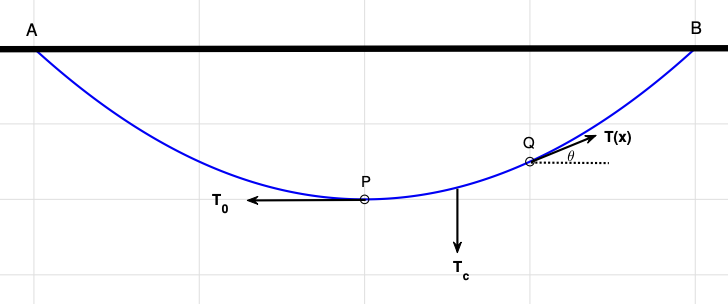
\includegraphics[scale=0.7]{Schema of Catenary.png}
  \caption{Schema of Catenary}
\end{figure}
\begin{solution}
  We consider an arbitrary piece of the chain \(PQ\), define \(\bf{T}(x)\) the tangential force, \(\bf{T_c}\) the weight, and \(\theta\) the angle with horizontal, as shown. We now balance the force and come up with a differential equation to solve.
  
  %EXT challenge 2
\end{solution}

%=========================================================
% \section{Series and differential equations}
% \subsection{Differential equations}

% %----------------------------------------------------
% \subsection{Power series}
% We assume the notion of series and power series is familiar as they have been introduced in the analysis course. Here is a reminder of radius of convergence and its ratio/root test.

% \begin{definition}[Radius of convergence]
%   The radius of convergence \(R\in [0,\infty]\) for a power series is such that the series converges \emph{absolutely} for \(|z|<R\) and diverges if \(|z|>R\). Alternatively,
%   \[R=\sup\left\{|z|:\sum_{n=1}^\infty a_nz^n \text{ converges}\right\}\]
%   if the set is bounded, or \(+\infty\) otherwise.
% \end{definition}
% Note that the case \(|z|=R\) needs to be examined separately.

% We see that the ratio and root test are particular useful for evaluating series.
% \begin{theorem}[Ratio and root test for series]
%   For power series \(\sum_{n=1}^\infty a_nz^n\), if \(|\frac{a_{n+1}}{a_n}| \to a\) or \(|a_n|^{1/n}\to a\) as \(n\to\infty\), then \(R=1/a\).
% \end{theorem}
% Note that if \(a=0\) then \(R=+\infty\).

% It turns out that we can differentiate and integrate power series just like polynomials (term by term) as long as we are within the radius of convergence.
% \begin{theorem}[Calculus of power series]
%   Let \(f(x)=\sum_{n=0}^{\infty}a_nx^n\) be a power series with radius of convergence \(R\). Then for \(|x|<R\), we have
%   \begin{align*}
%     f'(x)=\sum_{n=0}^{\infty}(n+1)a_{n+1}x^n && \int f(x)\,dx=\sum_{n=0 }^{\infty}\frac{a_nx^{n+1}}{n+1}
%   \end{align*}
% \end{theorem}
% In fact, we can differentiate/integrate it as many times as we want, so as long as \(|x|<R\), we can write the \(k\)th derivative of a power series \(y\) as 
% \[y^{(k)}=\sum_{n=k}^{\infty}\frac{n!}{(n-k)!}a_nx^{n-k}=\sum_{n=0}^{\infty}\frac{(n+k)!}{n!}a_{n+k}x^n\]

% With these information, we may find the power series solution of differential equations by substituting in and equating coefficients 

% \begin{exercise}
%   Find the power series solution to the system 
%   \[y'=1+y^2,\quad y(0)=0\]
% \end{exercise}
% \begin{solution} 
  
% \end{solution}

% %----------------------------------------------------
% \subsection{Taylor series}
% \begin{definition}[Taylor and Maclaurin series]
%   The Taylor series of \(f(x)\) about \(x=x_0\) is given by
%   \[f(x)=\sum_{n=0}^{\infty}\frac{f^{(n)}(x_0)}{n!}(x-x_0)^n\]
%   It is a Maclaurin series if \(x_0=0\).
% \end{definition}

%=========================================================
\section{Fourier Series and Fourier Transform}
\subsection{Fourier Series}
The Fourier series is a useful way to express periodic function as a discrete sum of complex exponential, especially when solving (partial) differential equations. It is used widely in many area of physics and engineering.

\begin{definition}[Periodic function]
  A function \(f(x)\) has period \(T\) (i.e. \(T\)-periodic) if \(f(x)=f(x+T)\) for all \(x\).
\end{definition}
\begin{definition}[Extension]
  Suppose function \(f(x),g(x)\) has domain \(D_1,D_2\) respectively. Then \(g\) is an extension of \(f\) if \(D_1\subset D_2\) and \(f(x)=g(x)\) for all \(x\in D_1\).
\end{definition}
It is common to define \(f(\xi)=\frac{1}{2}(f(\xi^+)+f(\xi^-))\) at any discontinuities, the average of the left and right values.

\begin{theorem}[Fourier series]
  Suppose a function \(f(x)\) defined on \([a,b]\) is integrable. Let \(L:=b-a\), then 
  \[F(x)=\sum_{n=0}^{\infty}c_n e^{i2\pi nx/L}\]
  where
  \[c_n=\frac{1}{L}\int_{a}^{b}f(x)e^{-i2\pi nx/L}\,dx\]
  and \(F(x)\) is a periodic extension to \(f(x)\) with period \(L\). We say \(F\) is the fourier series of \(f\) and \(c_n\) the Fourier coefficients of \(f\).
\end{theorem}

We may use Euler's formula \(e^{ix}=\cos(x)+i\sin(x)\) to give a trigonometric form of the Fourier series above:
\[F(x)=\frac{1}{2}a_0+\sum_{n=1}^{\infty}a_n\cos(\frac{2\pi nx}{L})+b_n\sin(\frac{2\pi nx}{L})\]
where
\[a_n=\frac{2}{L}\int_{a}^{b}f(x)\cos(\frac{2\pi nx}{L})\,dx\]
\[b_n=\frac{2}{L}\int_{a}^{b}f(x)\sin(\frac{2\pi nx}{L})\,dx\]

This comes in handy when \(f(x)\) is either even, \(f(x)=f(-x)\) or odd, \(f(x)=-f(-x)\). In the even case, we have \(b_n=0\) for all \(n\) and \(a_n=0\) for the odd case.

\begin{theorem}[Fourier theorem]
  If \(f,g\) has the same Fourier coefficients, then \(f\) and \(g\) are equal.
\end{theorem}\

\begin{theorem}[Riemann-Lebesgue lemma]
  If \(f(x)\) is integrable on \([a,b]\), then
  \[I_\lambda = \int_{a}^{b}f(x)\sin(\lambda x)\,dx\]
  tends to zero as \(\lambda\) tends to infinity.
\end{theorem}

\begin{theorem}[Parseval's theorem]
  For \(f\) an integrable function (and \(f^2\)) with Fourier series described trigonometric as above, we have
  \[\frac{1}{\pi}\int_{-\pi}^{\pi}(f(x)^2)\,dx=\frac{a_0^2}{2}+\sum_{n=1}^{\infty}(a_n^2+b_n^2)\] 
\end{theorem}

Fourier series holds many similar to Fourier transform discussed in next chapter (which is more important).

\subsection{Fourier transform}
A natural question to ask now is what would happen to Fourier series when the interval is \([-\infty,\infty]\) instead. It turns out by taking the limits we have an integral formula that can be applied to any (non-periodic) function, decomposing them into frequency components.

\begin{theorem}[Fourier transform]
  For an integrable function \(f(x)\), we have the following Fourier transform pair:
  \[\hat{f}(\omega)=\cal{F}\{f(x)\}=\int_{-\infty}^{\infty}f(x)e^{-i\omega x}\,dx\]
  \[f(x)=\cal{F}^{-1}\{\hat{f}(\omega)\}=\frac{1}{2\pi}\int_{-\infty}^{\infty}\hat{f}(\omega)e^{i\omega x}\,d\omega\]
\end{theorem}
\begin{proof}
  
\end{proof}
Here \(\cal{F}\{f(x)\}\) is the Fourier transform of \(f\), analogus to the Fourier coefficients in Fourier series. Applying the inverse Fourier again give back to original function.
\[\cal{F}^{-1}\{\cal{F}\{f(x)\}\}=\cal{F}\{\cal{F}^{-1}\{f(x)\}\}=f(x)\]

Similar to Fourier series, we also have a sine and cosine Fourier transform for odd and even function. Define
\[\hat{f}_c(\omega)=\int_{0}^{\infty}f(x)\cos(\omega x)\,dx\]
\[\hat{f}_s(\omega)=\int_{0}^{\infty}f(x)\sin(\omega x)\,dx\]
It is easy to see that
\[\hat{f}_c(\omega)=2\hat{f}(\omega),\:\hat{f}_s(\omega)=-2i\hat{f}(\omega)\]
In addition, the inverse transform is given by
\[f(x)=\frac{2}{\pi}\int_{0}^{\infty}\hat{f}_c(\omega)\cos(\omega x)\,dx,\; f(x)=\frac{2}{\pi}\int_{0}^{\infty}\hat{f}_s(\omega)\sin(\omega x)\,dx\]

Also useful to keep in mind that
\[2\cos(x)=e^{ix}+e^{-ix},\: 2i\sin(x)=e^{ix}-e^{-ix}\]

Just like Fourier series, we have that
\begin{theorem}[Uniqueness]
  If \(\cal{F}\{f(x)\}=\cal{F}\{g(x)\}\) for all \(x\), then \(f(x)=g(x)\) for all \(x\).
\end{theorem}

\begin{definition}[Complex conjugate of function]
  For a function \(f(x)\) defined over \(\C\), its complex conjugate \(f^*(x)\) is the function whose values are the complex conjugates of \(f(x)\), i.e. for all \(x\),
  \[f^*(x)=(f(x))^*\]
\end{definition}

\begin{proposition}[Properties of Fourier transform]
  For \(f,g\) integrable function, we have
  \begin{itemize}
    \item (Linearity) For \(a,b\in \C\), 
    \[\cal{F}\{af(x)+bg(x)\}=a\hat{f}(\omega)+b\hat{g}(\omega)\]
    \[\cal{F}^{-1}\{a\hat{f}(\omega)+b\hat{g}(\omega)\}=af(x)+bg(x)\]
    \item (Time scaling) For \(a\neq 0,a\in\R\),
    \[\cal{F}\{f(ax)\}=\frac{1}{|a|}\hat{f}(\frac{\omega}{a})\]
    Let \(a=-1\) leads to the time inversal property \(\cal{F}\{f(-x)\}=\hat{f}(-\omega)\).
    \item (Translation/Time shifting) For \(x_0\in\R\),
    \[\cal{F}\{f(x-x_0)\}=e^{-i\omega x_0}\hat{f}(\omega)\]
    \item (Modulation/Frequency shifting) For \(\omega_0\in\R\),
    \[\cal{F}\{e^{i\omega_0x}f(x)\}=\hat{f}(\omega-\omega_0)\]
    \item (Symmetry/Duality) Suppose \(\cal{F}\{f(x)\}=\hat{f}(\omega)\), we have 
    \[\cal{F}\{\hat{f}(\omega)\}=2\pi f(-x)\]
    \item (Conjugation)
    \[\cal{F}\{f^*(x)\}=\hat{f}^*(-\omega)\]
  \end{itemize}
  And some other minor properties
  \begin{itemize}
    \item \[\cal{F}\{\diff[n]{f}{x}\}=(i\omega)^n\hat{f}(\omega), \;\; \cal{F}\{\diff[n]{\hat{f}}{\omega}\}=(-ix)^nf(x)\]
    \item \[\int_{-\infty}^{x}f(t)\,dt=\frac{\hat{f}(\omega)}{i\omega}+\pi\hat{f}(0)\delta(\omega)\]
    \item \[\cal{F}\{x^nf(x)\}=i^n\diff[n]{\hat{f}}{\omega}\]
  \end{itemize}
\end{proposition}

\begin{problem}
  Find the Fourier transform of the Gaussian distribution given by \[f(x)=\frac{1}{\sigma\sqrt{2\pi}}e^{\frac{-x^2}{2\sigma^2}}\]
  Note that the Gaussian distribution is normalised, i.e. \(\int_{-\infty}^{\infty}f(x)\,dx=1\).
\end{problem}
\begin{solution}
  Consider 
  \[\diff{f}{x}=-\frac{x}{\sigma^2}f(x)\]
  Hence
  \[\cal{F}\{\diff{f}{x}\}=-\frac{1}{\sigma^2}\cal{F}\{xf(x)\}=\frac{-i}{\sigma^2}\diff{\hat{f}}{\omega}\]
  But we also have 
  \[\cal{F}\{\diff{f}{x}\}=i\omega\hat{f}(\omega)\]
  Hence we arrive at a separable differential equation
  \[\frac{\rm{d}\hat{f}}{\hat{f}}=-\omega\sigma^2\]
  Integrating both sides with respect to \(\omega\) gives
  \[\ln(\hat{f})=-\frac{\omega^2\sigma^2}{2}+c\]
  \[\hat{f}(\omega)=ae^{-\frac{\omega^2\sigma^2}{2}}\]
  Since Gaussian is normalised, we have \(\hat{f}(0)=\int_{-\infty}^{\infty}f(x)\,dx=1\), hence \(a=1\).
\end{solution}

\subsection{Convolution and energy theorem}
% does it have to be defined over all reals
\begin{definition}[Convolution]
  For \(f,g\) integrable functions defined over \(\R\), the convolution of \(f,g\) is given by
  \[f(x)*g(x)=\int_{-\infty}^{\infty}f(x-u)g(u)\,du\]
\end{definition}

Here is an very important theorem.
\begin{theorem}[Convolution theorem]
  For \(f,g\) integrable functions defined over \(\R\), we have
  \[\cal{F}\{f(x)*g(x)\}=\hat{f}(\omega)\hat{g}(\omega)\]
  \[\cal{F}\{f(x)g(x)\}=\frac{1}{2\pi}\hat{f}(\omega)*\hat{g}(\omega)\]
\end{theorem}
\begin{proof}
  
\end{proof}

\begin{proposition}[Convolution properties]
  Convolution behaves algebraically like multiplication. Given \(f,g\), we have
  \begin{itemize}
    \item (Commutative)
    \item (Associative)
    \item (Distributive over addition)
    \item (Delta as identity)
    \item (Bilinear)
  \end{itemize}
\end{proposition}

\begin{theorem}[Paresval's/Energy theorem]
  For \(f(x)\) an integrable function defined over \(\C\), we have
  \[\int_{-\infty}^{\infty}f(x)f^*(x)\,dx=\frac{1}{2\pi}\int_{-\infty}^{\infty} \hat{f}(\omega)\hat{f}^*(\omega)\,d\omega\]
\end{theorem}

\begin{theorem}[Mean value theorem for integral]
  If \(f(x)\) is continuous on \([a,b]\), then 
  \[\int_{a}^{b}f(x)\,dx=(b-a)f(\bar{x})\]
  for at least one \(\bar{x}\in[a,b]\).
\end{theorem}

\begin{definition}[Dirac delta function]
  Consider the following step function
  \[f_k(x)=\begin{cases}
    k/2, & |x|<1/k\\
    0, & |x|\geq 1/k
  \end{cases}\]
  The Dirac delta function is defined to be
  \[\delta(x)=\lim_{k\to\infty}f_k(x)\]
\end{definition}
This is sometimes called the unit impulse function. Effectively, \(\delta(x)\) is infinite at \(x=0\) and zero at everywhere else. The key property however, is that its integral (area under the curve) is one as it is ture for all \(k\).

The delta function is most useful in how it interacts with other functions.
\begin{proposition}[Sifting property of Dirac delta]
  For \(f(x)\) a continuous function over \(\R\), we have
  \[\int_{-\infty}^{\infty}f(x)\delta(x-a)\,dx=\delta(a)\]
\end{proposition}
It is easy to show using the sifting property that \(\cal{F}\{\delta(x)\}=e^{i\omega 0}=1\). Hence using the inversion formula, and noticing \(\delta(x)\) is an even function, we have an useful alternative expression for the delta function:
\[\delta(x)=\frac{1}{2\pi}\int_{-\infty}^{\infty}e^{\pm i\omega x}\,d\omega\]
Of course, we can have \(\omega\) as the variable also. 
\begin{definition}[Heaviside step function]
  The Heaviside step function is defined as
  \[H(x)=\begin{cases}
    1,&x>0\\0,&x<0
  \end{cases}\]
\end{definition}

Here are a few common Fourier transform pairs:
\begin{itemize}
  \item \(f(x)=\delta(x), \hat{f}(\omega)=1\)
  \item \(f(x)=H(x),\hat{f}(\omega)=\frac{1}{i\omega}+\pi\delta(\omega)\)
  \item \(f(x)=\rm{sgn}(x),\hat{f}(\omega)=\frac{2}{i\omega}\)
  \item \(f(x)=e^{-ax}H(x),\hat{f}(\omega)=\frac{1}{a+i\omega}\)
  \item \(f(x)=e^{-a|x|},\hat{f}(\omega)=\frac{2a}{a^2+\omega^2}\)
  \item \(f(x)=\begin{cases}
    1, & |x|<d\\ 0, & |x|>d
  \end{cases}, \hat{f}(\omega)=\frac{2}{\omega}\sin(\omega d)\)
\end{itemize}

\section{Ordinary Differential Equations}
\subsection{First and second order ODEs}
The following are two common ways to solve first order equations.
\begin{theorem}[Separable equation]
  If a differential equation can be written as \[\diff{y}{x}=f(x)g(y)\] and \(g(y)\neq 0\), then we may solve it by separating variables
  \[\int \frac{dy}{g(y)} = \int f(x)\,dx\]
\end{theorem}

\begin{theorem}[Integrating factor]
  If a differential equation can be written as \[\diff{y}{x}+p(x)y=q(x)\] then set the integrating factor to be \(I(x)=\exp(\int p(x)\,dx)\) (costant = 0), we have 
  \[\diff{}{x}I(x)y=I(x)q(x)\]
  \[y=\frac{1}{I(x)}\int I(x)q(x)\,dx\]
\end{theorem}

Thre are some common substitution techniques 

\textbf{Second order}
We may simplify the second order in some special cases. Suppose the genearl explicit form 
\[\diff[2]{y}{x}=F(x,y,\diff{y}{x})\]
\begin{itemize}
  \item depends on only \(x\). Then we can simply integrate directly twice.
  \item depends on \(x,\diff{y}{x}\). Then substitute \(u=\diff{y}{x}\) would convert it to a first order in \((x,u)\).
  \item depends on \(y,\diff{y}{x}\). Substitute \(u=\diff{y}{x}\) convert it to a first order in \((y,u)\) as
  \[\diff{u}{x}=\diff{u}{y}\diff{y}{x}=u\diff{u}{y}=\diff{}{y}\left(\frac{u^2}{2}\right)\]
\end{itemize}

In the case that the equation is linear constant coefficients, we have the following
\begin{proposition}
  
\end{proposition}

\subsection{Linear ODEs}

\end{document}